\documentclass{beamer}
\usepackage[utf8]{inputenc}
\usepackage[T1]{fontenc}
\usepackage[english]{babel}
\usepackage{hyperref}
\usepackage{outlines}
\usepackage{graphicx}
\usepackage{algorithm}
\usepackage{algorithmic}
\usepackage{amsmath,amssymb}
\usepackage{moresize}
\usepackage{tikz}
\usetikzlibrary{overlay-beamer-styles}
\usepackage{microtype}
\usepackage[
  backend=biber,
  style=alphabetic,
]{biblatex}
\usepackage{latexsym,multicol,booktabs,calligra}
\usepackage{listings,stackengine}
\usepackage[table,dvipsnames]{xcolor}
\usepackage{cancel}
\renewcommand{\figurename}{Figure}
\renewcommand{\algorithmname}{Algorithm}

\usepackage{SHU}
\setbeamersize{text margin left=7mm, text margin right=7mm}
\def\cmd#1{\texttt{\color{red}\footnotesize $\backslash$#1}}
\def\env#1{\texttt{\color{blue}\footnotesize #1}}
\definecolor{deepblue}{rgb}{0,0,0.5}
\definecolor{deepred}{rgb}{0.6,0,0}
\definecolor{deepgreen}{rgb}{0,0.5,0}
\definecolor{halfgray}{gray}{0.55}
\definecolor{nus-orange}{RGB}{239,124,0}
\definecolor{nus-white}{RGB}{255,255,255}
\definecolor{nus-blue}{RGB}{0,61,124}
\definecolor{nus-black}{RGB}{0,0,0}

\lstset{
  language=SQL,
  basicstyle=\ttfamily\footnotesize,
  keywordstyle=\bfseries\color{nus-blue},
  emphstyle=\ttfamily\color{nus-blue},
  stringstyle=\color{deepgreen},
  numbers=left,
  numberstyle=\small\color{halfgray},
  rulesepcolor=\color{nus-orange},
  frame=shadowbox,
  showstringspaces=false,
  breaklines=true,
  breakatwhitespace=true,
  keepspaces=true,
  columns=flexible,
  upquote=true
}

\author{\href{https://pratik2358.github.io/}{Pratik Karmakar}}
\title{IT5008: Tutorial 4 — Aggregate and Nested Queries}
\institute{
  School of Computing,\\
  National University of Singapore
}
\date{AY25/26 S1}

\begin{document}

\begin{frame}
  \titlepage
  \begin{figure}[htpb]
    \begin{center}
      
\includegraphics[keepaspectratio, scale=0.18]{nus-logo.png}
    \end{center}
  \end{figure}
\end{frame}

\section{Setup}
\begin{frame}{Scenario}
\small
Students at the \textbf{National University of Ngendipura (NUN)} buy, lend, and borrow books.\\
NUNStA commissions \emph{Apasaja Private Limited} to implement an online book exchange system that records:
\begin{itemize}\itemsep3pt
  \item Students: name, faculty, department, \textbf{email} (identifier), join year.
  \item Books: title, authors, publisher, year, edition, \textbf{ISBN10}, \textbf{ISBN13}.
  \item Loans: \texttt{borrowed} date, \texttt{returned} date (may be \texttt{NULL}).
\end{itemize}
Auditing preserves data for graduated students and copies with loan records. \\
This tutorial uses the schema/data created in “Creating and Populating Tables”.
\end{frame}

\begin{frame}{Important Constraints}
\Large
\begin{block}{This tutorial:}
Focus on \textbf{aggregate} and \textbf{nested} queries.\\
Practice writing equivalent formulations and ensure readability.
\end{block}
\end{frame}

\section{Questions}
\begin{frame}{Questions — Aggregate}
\footnotesize
\textbf{1.\ Aggregate Queries}
\begin{enumerate}
  \item[(a)] How many loans involve an owner and a borrower from the same department?
  \item[(b)] For each faculty, print the number of loans that involve an owner and borrower from this faculty.
  \item[(c)] What are the average and standard deviation of loan duration (in days)?
\end{enumerate}
\end{frame}

\begin{frame}{Questions — Nested}
\footnotesize
\textbf{2.\ Nested Queries}
\begin{enumerate}
  \item[(a)] Print titles of books that have never been borrowed (use nested query).
  \item[(b)] Print names of students who own a copy of a book never lent.
  \item[(c)] For each department, print names of students who lent the most.
  \item[(d)] Print emails and names of students who borrowed all books authored by Adam Smith.
\end{enumerate}
\end{frame}

\section{Solutions}
\begin{frame}[fragile]{1(a).\ Number of loans in same department}
\begin{lstlisting}
SELECT COUNT(*)
FROM loan l, student s1, student s2
WHERE l.owner = s1.email
  AND l.borrower = s2.email
  AND s1.department = s2.department;
\end{lstlisting}
\end{frame}

\begin{frame}[fragile]{1(b).\ Number of loans within faculty}
\begin{lstlisting}
SELECT d1.faculty, COUNT(*)
FROM loan l, student s1, student s2,
     department d1, department d2
WHERE l.owner = s1.email
  AND l.borrower = s2.email
  AND s1.department = d1.department
  AND s2.department = d2.department
  AND d1.faculty = d2.faculty
GROUP BY d1.faculty;
\end{lstlisting}
\end{frame}

\begin{frame}[fragile]{1(c).\ Average and Stddev of Loan Duration}
\textbf{Alternative \#1 (inline CASE):}
\begin{lstlisting}
SELECT CEIL(AVG((CASE
    WHEN l.returned ISNULL
      THEN CURRENT_DATE
    ELSE l.returned END) - l.borrowed + 1)),
  CEIL(STDDEV_POP((CASE
    WHEN l.returned ISNULL
      THEN CURRENT_DATE
    ELSE l.returned END) - l.borrowed + 1))
FROM loan l;
\end{lstlisting}
\end{frame}

\begin{frame}[fragile]{1(c).\ Alternative Query (Subquery)}
\begin{lstlisting}
SELECT CEIL(AVG(temp.duration)),
       CEIL(STDDEV_POP(temp.duration))
FROM (
  SELECT ((CASE
     WHEN l.returned ISNULL THEN CURRENT_DATE
     ELSE l.returned END) - l.borrowed + 1) AS duration
  FROM loan l
) AS temp;
\end{lstlisting}
\end{frame}

\begin{frame}[fragile]{2(a).\ Books never borrowed}
\textbf{Option \#1 (NOT IN):}
\begin{lstlisting}
SELECT b.title
FROM book b
WHERE b.ISBN13 NOT IN (
  SELECT l.book
  FROM loan l);
\end{lstlisting}
\end{frame}

\begin{frame}[fragile]{2(a).\ Alternative (<> ALL)}
\begin{lstlisting}
SELECT b.title
FROM book b
WHERE b.ISBN13 <> ALL (
  SELECT l.book
  FROM loan l);
\end{lstlisting}
\end{frame}

\begin{frame}[fragile]{2(b).\ Students who never lent their copy}
\begin{lstlisting}
SELECT s.name
FROM student s
WHERE s.email IN (
  SELECT c.owner
  FROM copy c
  WHERE NOT EXISTS (
    SELECT *
    FROM loan l
    WHERE l.owner = c.owner
      AND l.book = c.book
      AND l.copy = c.copy));
\end{lstlisting}
\end{frame}

\begin{frame}[fragile]{2(c).\ Top lenders in each department}
\begin{lstlisting}
SELECT s.department, s.name, COUNT(*)
FROM student s, loan l
WHERE l.owner = s.email
GROUP BY s.department, s.email, s.name
HAVING COUNT(*) >= ALL (
  SELECT COUNT(*)
  FROM student s1, loan l1
  WHERE l1.owner = s1.email
    AND s.department = s1.department
  GROUP BY s1.email);
\end{lstlisting}
\end{frame}

\begin{frame}[fragile]{2(d).\ Borrowed all Adam Smith books}
\begin{lstlisting}
SELECT s.email, s.name
FROM student s
WHERE NOT EXISTS (
  SELECT *
  FROM book b
  WHERE authors = 'Adam Smith'
    AND NOT EXISTS (
      SELECT *
      FROM loan l
      WHERE l.book = b.ISBN13
        AND l.borrower = s.email));
\end{lstlisting}
\end{frame}

\begin{frame}[fragile]{2(d).\ Borrowed all Adam Smith books}
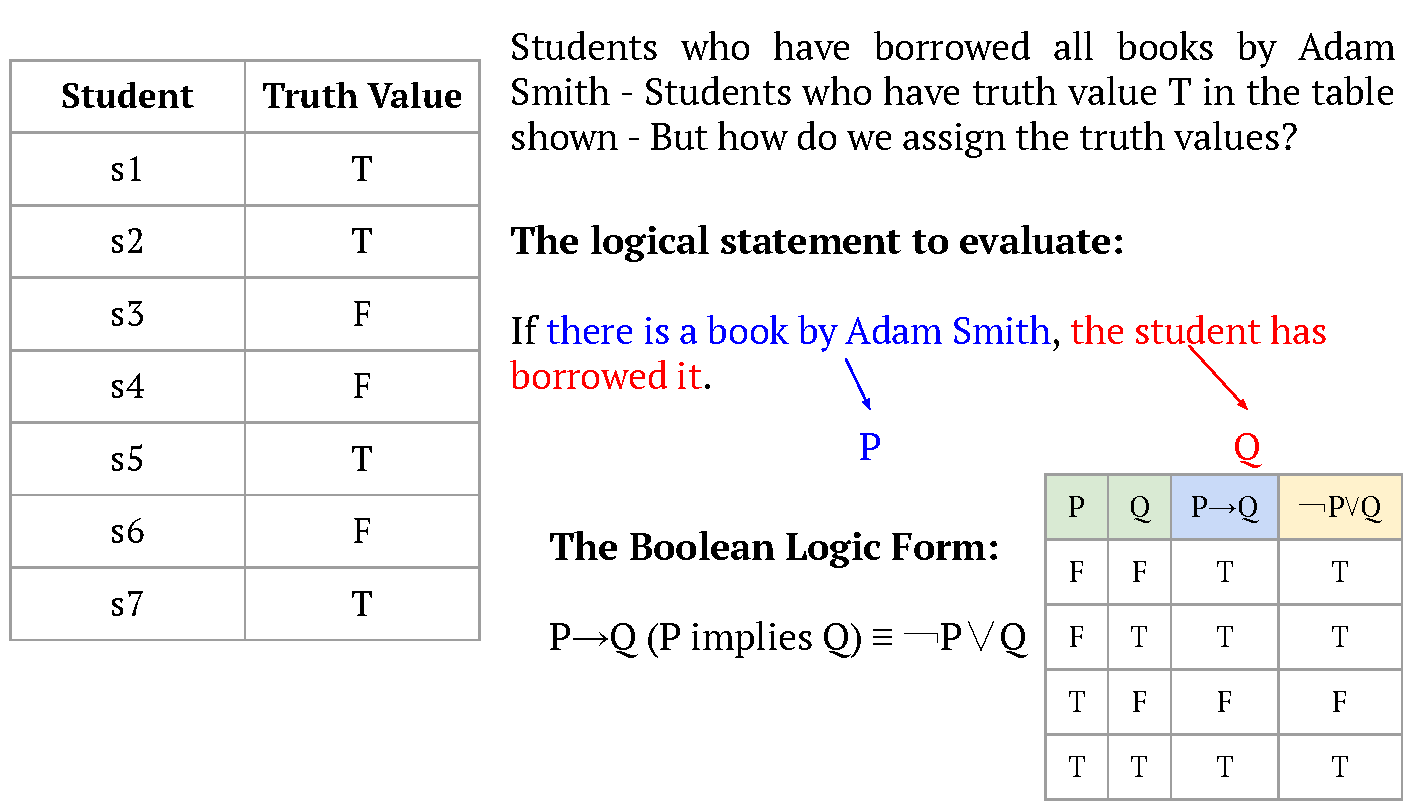
\includegraphics[scale = 0.45]{tut_07_images/tut_07_02.pdf}
\end{frame}

\begin{frame}[fragile]{2(d).\ Borrowed all Adam Smith books}
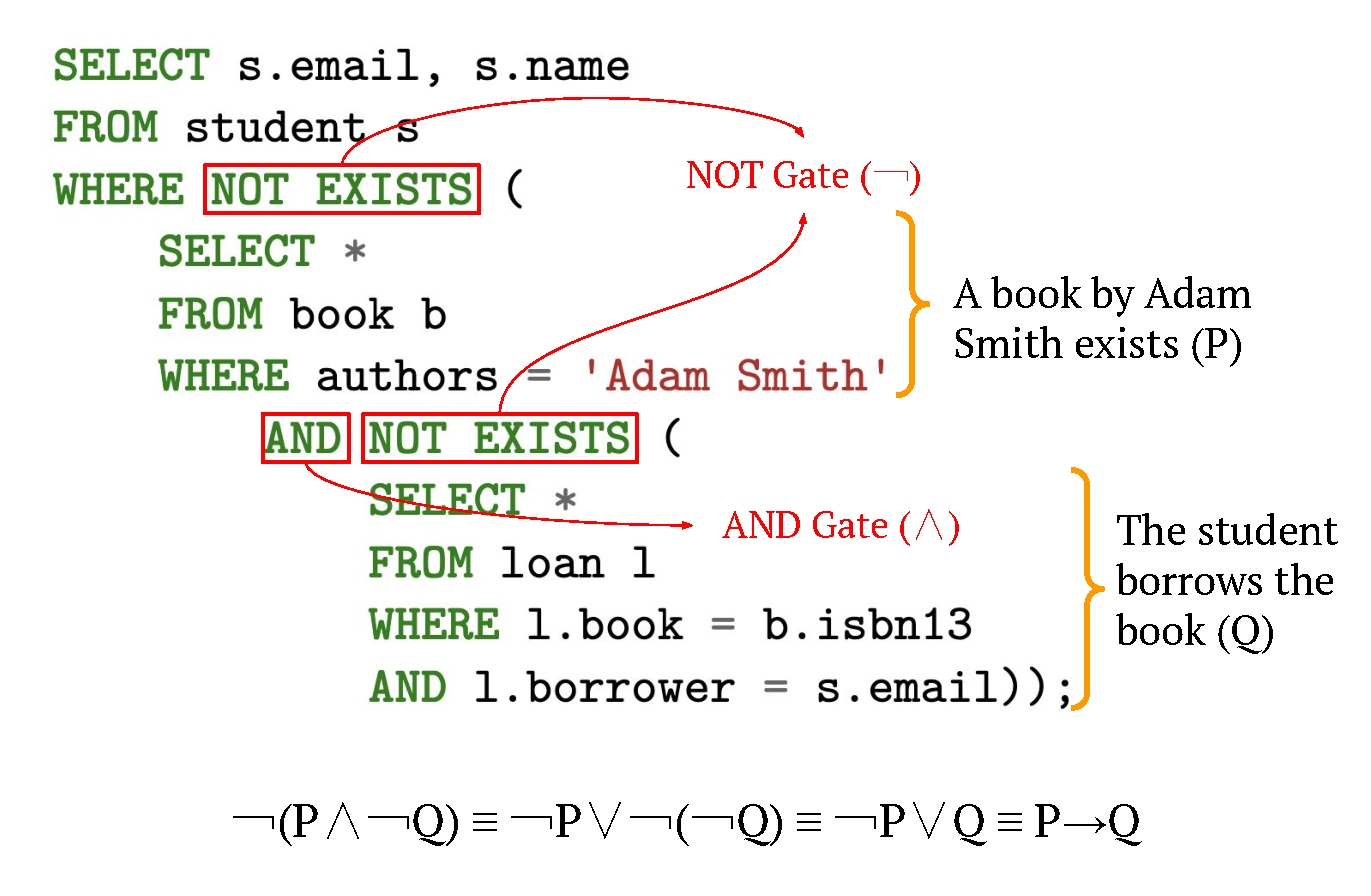
\includegraphics[scale = 0.45]{tut_07_images/tut_07_01.pdf}
\end{frame}

\section{Guidelines}
\begin{frame}{Guidelines \& Marking Tips}
\small
\begin{itemize}\itemsep4pt
  \item \textbf{No hardcoding.} Queries must work on any dataset consistent with the schema.
  \item Use \textbf{quantifiers} (\texttt{ALL}/\texttt{ANY}) explicitly in subqueries.
  \item Avoid using \textbf{TOP N / LIMIT} for max/min — prefer ALL with GROUP BY.
  \item Be cautious of duplicate elimination; use \texttt{DISTINCT} only when needed.
  \item Write queries in \textbf{readable, indented style}.
\end{itemize}
\end{frame}

\begin{frame}
\begin{center}
Questions?\\
Drop a mail at: pratik.karmakar@u.nus.edu
\end{center}
\end{frame}

\end{document}